\documentclass{article}
\usepackage[fleqn]{amsmath}
\usepackage{amssymb,graphicx,color,graphicx,slashed, microtype, parskip, enumitem, extarrows, needspace}
%\usepackage[utf8x]{inputenc}
\usepackage[top=1.5cm, bottom=1.5cm, right=6cm, left=1.5cm, heightrounded, marginparwidth=5cm, marginparsep=0.5cm]{geometry}

\hbadness = 10000
\hfuzz=100pt 
    
\usepackage{marginnote}
\renewcommand*{\marginfont}{\footnotesize}

\usepackage{hyperref}
\hypersetup{colorlinks=true, urlcolor=NavyBlue, bookmarksdepth=3}

\makeatletter\newcommand{\@minipagerestore}{\setlength{\parskip}{\medskipamount}}\makeatother

% =============== Index ===========================

\usepackage[nonewpage]{imakeidx}
\makeindex

% =============== Color Definitions ===============
    
\usepackage[svgnames]{xcolor}
\colorlet{ColorTitle}{Black}
\colorlet{ColorSectionName}{Black}
\colorlet{ColorBoxFG}{Gray}
\colorlet{ColorBoxText}{Black}
\colorlet{ColorBoxBG}{White}


% =============== Title Style ===============
    
\usepackage{titling} % Allows custom title configuration
    
\newcommand{\HorRule}{\color{ColorTitle}\rule{\linewidth}{1pt}} % Defines the gold horizontal rule around the title
    
\pretitle{
    \vspace{-50pt} % Move the entire title section up
    \HorRule\vspace{9pt} % Horizontal rule before the title
    \fontsize{27}{36}\usefont{OT1}{phv}{b}{n}\selectfont
    \color{ColorTitle} % Text colour for the title and author(s)
}
    
\posttitle{\par\vskip 15pt} % Whitespace under the title
    
\preauthor{\fontsize{17}{0}\usefont{OT1}{phv}{m}{n}\selectfont\color{ColorTitle}} % Anything that will appear before \author is printed
    
\postauthor{\par\HorRule}

\newcommand{\COURSENAME}{\href{http://phyw.people.ust.hk/teaching/PHYS2022-2015/}{\textcolor{black}{PHYS 2022}}}
\newcommand{\YW}{\href{http://phyw.people.ust.hk/}{\textcolor{black}{Yi Wang}}}
\newcommand{\PHYS}{\href{http://physics.ust.hk}{\textcolor{black}{Department of Physics}}}
\newcommand{\HKUST}{\href{http://www.ust.hk/}{\textcolor{black}{HKUST}}}
\author{\COURSENAME, \YW, \PHYS, \HKUST}

\date{}

% =============== Section Name Style ===============
    
\usepackage{titlesec}
    
\titleformat{\section}
    {\fontsize{15}{20}\usefont{OT1}{phv}{b}{n}\color{ColorSectionName}}
    {\thesection}{1em}{}
    %[{\vspace{0.2cm}\titlerule[0.8pt]}]
    
\titleformat{\subsection}
    {\fontsize{14}{20}\usefont{OT1}{phv}{m}{n}\color{ColorSectionName}}
    {\thesubsection}{1em}{}
    
\titleformat{\subsubsection}
    {\fontsize{12}{20}\usefont{OT1}{phv}{m}{n}\color{ColorSectionName}}
    {}{0em}{}
      
\setcounter{secnumdepth}{4}
        
% =============== Box Style ===============
    
\usepackage[most]{tcolorbox}
    
\newtcolorbox{tbox}[1]{
    colback=ColorBoxBG, colframe=ColorBoxFG, coltext=ColorBoxText,
    sharp corners, enhanced, breakable, parbox=false,
    before skip=1em, after skip=1em,
    title={#1}, fonttitle=\usefont{OT1}{phv}{b}{n}, 
    attach boxed title to top left={yshift=-0.1mm}, boxed title style={sharp corners, colback=ColorBoxFG, left=0.405cm},
    rightrule=-1pt,toprule=-1pt, bottomrule=-1pt
}

\newtcolorbox{mtbox}[1]{
    colback=ColorBoxBG, colframe=ColorBoxFG, coltext=ColorBoxText,
    sharp corners, enhanced, breakable, parbox=false,
    before skip=1em, after skip=1em,
    title={#1}, fonttitle=\usefont{OT1}{phv}{b}{n},
    attach boxed title to top left={yshift=-0.1mm}, boxed title style={sharp corners, colback=ColorBoxFG, left=0.15cm},
    rightrule=-1pt,toprule=-1pt, bottomrule=-1pt, 
    left=0.5em
}

% =============== tikz has to be loaded after xcolor
\usepackage{tikz}

\newcommand*\enumlabel[1]{\tikz[baseline=(char.base)]{
			\node[shape=rectangle,inner sep=2pt,fill=ColorBoxFG] (char) 
			{\fontsize{7}{20}\usefont{OT1}{phv}{b}{n}{\textcolor{ColorBoxBG}{#1}}};}}

% =============== Useful shortcuts ===============

\newcommand\wref[1]{{\hypersetup{linkcolor=white}\ref{#1}}}  

\newcommand{\textbox}[2]{
    \begin{tbox}{#1}
        #2
    \end{tbox}
}

\newcommand{\mtextbox}[2]{\marginnote{
    \begin{mtbox}{#1}
        #2
    \end{mtbox}}
}

\newcommand{\mnewline}{\vspace{0.5em}\newline}

\newcommand{\titem}[1]{
    \begin{itemize}[label=\color{ColorBoxFG}$\blacktriangleright$, leftmargin=0mm, labelsep=0.27cm, topsep=0.5em
        %, itemsep=1ex
        ]
        #1
    \end{itemize}
}

\newcommand{\mtitem}[1]{
    \begin{itemize}[label={\color{ColorBoxFG}$\blacktriangleright$}, leftmargin=0mm, labelsep=1mm, topsep=0.5em
        %, itemsep=1ex
        ]
        #1
    \end{itemize}
}

\newcommand{\itembox}[3]{
    \begin{tbox}{#1}
        #2
        \titem{#3}
    \end{tbox}
}

\newcommand{\mitembox}[3]{
    \marginnote{
    \begin{mtbox}{#1}
        #2
        \mtitem{#3}
	\end{mtbox}
    }
}

\newcommand{\tenum}[1]{
    \begin{enumerate}[label=\protect\enumlabel{\arabic*}, leftmargin=0mm, labelsep=0.265cm, topsep=0.5em
        %, itemsep=1ex
        ]
        #1
    \end{enumerate}
}

\newcommand{\enumbox}[3]{
    \begin{tbox}{#1}
        #2
        \tenum{#3}
    \end{tbox}
}

\newcommand{\twocol}[5]{
    \begin{minipage}[t][][b]
        {#1\textwidth}
        #4        
    \end{minipage}
    \hspace{#2\textwidth}
    \begin{minipage}[t][][b]
        {#3\textwidth}
        #5
    \end{minipage}
}

\newcommand{\cg}[2]{
    \begin{center}
        \includegraphics[width=#1\textwidth]{#2}
    \end{center}
}

\newcommand{\tbar}{
    ~\newline
    {\color{ColorBoxFG}
    \hbox to 0.15\textwidth{\leaders\hbox to 5pt{\hss  \hss}\hfil} 
    \hbox to 0.7\textwidth{\leaders\hbox to 5pt{\hss . \hss}\hfil}}
    \mnewline
}

% =============== Filter unwanted warnings
\usepackage{silence}
\WarningsOff[tcolorbox]
\hbadness=1000000


\graphicspath{{3_fig/}}
\title{第三章\ 宇宙学}

\usepackage{ctex}
\begin{document}

\maketitle

\textbox{可理解的宇宙}{
    宇宙最复杂的东西就是其本身, 因为它包含了宇宙内一切事物的复杂性。 但是神奇的是爱因斯坦说过:

    “这个世界的最不可理解之处就这于它是可以理解的。”

    让我们试着来理解以下问题:

    \tenum{
        \item 在我们理解宇宙万物之前, 我们要如何理解最复杂的宇宙?
        \item 为什么夜空是黑色的?
        \mtextbox{奥伯斯佯谬的其他理解}{
            奥伯斯佯谬也有其他等效且深刻的理解方式:
            \mtitem{
                \item 在沿着视线无限小的圆锥体内, 存在一颗与太阳一样亮的星星。太阳整体最亮因为它占据了更大的视角。如果宇宙是无限的,我们的视线迟早会碰到一颗星星的表面。因此天空永远都和太阳一样亮。 
                \item 如果宇宙是静止且无限持续的,那么地球会达到与恒星的平衡,所以地球会与恒星表面一样热。
            }
        }
         
        
        这个问题的答案听上去很显然:因为夜晚没有阳光照射地球。但是其它恒星呢?为什么在其它恒星照射下,夜空不会跟白昼一样亮? 

        你可能会想: 它们离地球太远了。它们的光度会以$1/r^2$衰减,所以它们不会跟太阳一样亮。

        回答正确。但是在$r$处有多少恒星? 如果我们的宇宙在空间和时间上是同质且无限的,统计上来说,在$r$处的恒星数量会以$r^2$增长。所以为什么它们的光不会累计到像太阳一样亮?

        这个问题被称为奥伯斯佯谬。(迪格斯 1576, 奥伯斯 1823)。
    }
}

\section{宇宙动力学} 
\label{sec:dynamics-universe}

\textbox{宇宙学原理}{
    为了简化宇宙,设:

    宇宙总体来说是几乎同质且各向同性的。

    这就是宇宙学原理。
}

这个宇宙学原理已经出现过在牛顿的《自然哲学的数学原理》(1687)。然而,牛顿力学对宇宙学的研究充满了悖论。现代宇宙学的框架是建立在爱因斯坦广义相对论的基础上的。

在本节中,我们将继续用牛顿力学来谨慎地建立我们的宇宙理论。我们可以用广义相对论来验证探究的细节。

\textbox{遥远的星系全都在远离我们而去}{
    1920年代, 哈勃 (见勒梅特与其他天文学家的贡献) 从其他星系测量了光谱。已知发射光谱(回想原子的特征光谱), 通过测量已知光谱,运用红移现象可知这些星系沿视线的速率。

    结论显示遥远的星系全都在远离我们而去。 
}

\mtextbox{比光还快?}{
    宇宙膨胀的速度是不是比光速快?更精确地来说,足够遥远的物体能以比光速还快的速度离开我们吗?
    \tcblower
    是与否取决于我们如何来定义广义相对论的速度。 
    \mnewline
    定义速度为$dR(t)/dt$, 那么足够遥远的物体的确以比光速还快的速度离开我们。这个不是因为物体本身移动得快,而是因为物体之间出现了空间。这与狭义相对论并不相悖,因为两个邻近物体的速度(狭义相对论适用的地方)不会快于光速。
    \mnewline
    如果定义速度为移动物体的速度(本动速度),不考虑空间的膨胀,那么遥远物体的速度还是被光速所束缚。
}
\textbox{从哥白尼原理到膨胀的宇宙}{
    从哥白尼开始,人类开始意识到宇宙没有中心。但是,如果遥远星系都在离开我们,这是否意味着我们就在宇宙的中心? 

    不一定。想象一个膨胀的膜或者气球。无论你处在膜上或者气球上的任何一点,你都会发现邻近的点在离你而去。因此我们可以理解这个现象为宇宙正在膨胀。

    既然宇宙在膨胀,要如何来求扩张率呢?
    \tcblower
    想象一个充满无压力尘埃的宇宙。这些尘埃粒子在自己不运动的情况下 (既共动、本动),与宇宙一起膨胀。

    \cg{0.35}{cosmo_sphere}

    我们定义两套距离:共动距离和物理距离。从而在牛顿力学的框架内,量化宇宙的膨胀率。
    \titem{
        \item 物理距离$R(t)$是与实际物理测量相对应的两个物体之间实际距离。
        \item 共动距离$r$是以共动坐标系测量的。从而使共同运动的尘埃粒子在共动坐标系中具有固定的(即与时间无关的)坐标值。
    }
    共动坐标与物理坐标的关系式为
    $
        R(t) = a(t) r,
    $
    $a(t)$叫做\textbf{比例因子},用来量化时间对宇宙的相关性。 宇宙的膨胀率以哈勃参数量化:
    \begin{align}
        H(t) \equiv \frac{\dot a}{a} ~
    \end{align}
}

\needspace{0.2\textheight}
\mtextbox{尘埃与辐射}{
    例子:
    \mtitem{
        \item 无压力的尘埃:
        $p=0$。解\eqref{eq:continuous}可得$\rho \propto a^{-3}$。粒子密度稀释为$a^{-3}$,且每个粒子的能量为常数。
        \item 辐射:光子的密度$\propto a^{-3}$。但是每个光子的波长以$\lambda \propto a$拉伸。因此每个光子的能量与$1/a$成正比(量化的条件)。所以$\rho \propto a^{-4}$。这相当于$p=\rho/3$。
    }
    因为辐射比尘埃更快地被稀释,所以宇宙在膨胀的过程中由辐射主导转变为尘埃主导。 
}
\textbox{宇宙告诉我们物质是怎么被稀释的}{
    想象一个能量密度为$\rho$、压力为$p$的宇宙的组成部分(例如辐射、尘埃粒子)。$\rho$如何随时间演变?
    
    热学第一定律为$dE = TdS - pdV$。因为在同质的宇宙中不会传导热量,所以宇宙的膨胀是绝热的。因此$dS=0$。所以在宇宙的膨胀过程中,$dE/dt = p dV/dt$。此处的$V$是一个物理体积$V\propto a^3$。所以,    \begin{align}\label{eq:continuous}
        \frac{d(a^3\rho)}{dt}  = p \frac{da^3}{dt}
        \qquad\Rightarrow\qquad
        \dot \rho + 3H (\rho +p) = 0~
    \end{align}
    这被称为宇宙学的连续性方程,它告诉我们物质在宇宙的膨胀过程中是怎么被稀释的。
}

\textbox{宇宙里有什么物质?}{
    人类只知道宇宙组成的5\%(由能量组成来计算)。下图显示了人类已知和未知的物质。
    \cg{0.8}{components}
    \mtextbox{爱因斯坦的“大错误”}{
        爱因斯坦第一次用广义相对论来研究宇宙的时候,他发现宇宙要么膨胀要么收缩。他对这个状态并不满意,所以他在他的等式上加了一个宇宙学常数使宇宙如他所愿静止下来(1917)。 当哈勃在1920年代发现了宇宙的膨胀之后,爱因斯坦后悔他错过了发现宇宙膨胀的机会,所以他认为引入宇宙常数是他一生中最大的错误(1931)。可是在1998年,暗能量被发现,最简单的解释就是宇宙学常数(不一样的数值使宇宙以正加速度膨胀而不是静止)。
    }                     
    \titem{
        \item 已知物质:由核子与电子组成的物质(原子或者等离子)占据宇宙总能量的5\%。大部分原子和等离子以自由氢和自由氦的形式存在,小部分组成恒星。在我们已知的物质中,光的重量也占了极小的一部分(0.005\%)。
        \item 未知物质:观察显示宇宙里存在有暗物质(占大约25\%)和暗能量(占大约70\%)。我们并不知道它们到底是什么。但是从观察来看,我们知道它们大概的特性:暗物质的主要组成是几乎无压力的既$p\sim 0$,就跟原子物质一样,而且使吸引力变大。然而,暗能量的压力为$p\sim -\rho$。它有效提供了排斥引力,并且推动宇宙的加速膨胀阶段。
        }
}

\textbox{物质告诉我们宇宙是怎么膨胀的}{
    为了求$a(t)$的特性,想象一个质量为$m$、位于共动距离$r$(物理距离为$R(t)=a(t)r$)的尘埃粒子。它的能量守恒等式为
    \begin{align}\label{eq:pre-friedmann-1}
        \frac{m}{2} \left ( \frac{dR}{dt}  \right)^2 - \frac{GMm}{R} = E = \mathrm{constant}~
    \end{align}
    常数$E$由宇宙的初始状态决定。观察显示$E\simeq 0$,因此我们可以忽略它(不忽略为什么$E\simeq 0$)。

    这里的$M$为球体里面的质量:
    \mtextbox{球体外面的质量呢?}{
        因为每个球体的作用力都被抵消掉了,你可以说球体外面的力并不作用于我们的粒子$m$。实际上,这个陈述取决于宇宙边界的情况。这就是牛顿宇宙学的局限性。我们需要运用广义相对论从而使它不取决于边界的情况。
        }
    \begin{align}\label{eq:pre-friedmann-2}
        Mc^2 = \frac{4\pi R^3}{3} \rho~
    \end{align}
    将\eqref{eq:pre-friedmann-2}代入 \eqref{eq:pre-friedmann-1},可以得到弗里德曼方程(告诉我们宇宙是如何膨胀的):
    \begin{align}\label{eq:friedmann}
        H^2 = \frac{8\pi G \rho}{3c^2}~  
    \end{align}
    在牛顿宇宙学中,$p\neq 0$是无法求解的。这是因为牛顿重力没有定义压力是怎么影响引力的。因此在上述推导中,我们运用了一个充满尘埃的宇宙。运用广义相对论,我们可以证实\eqref{eq:friedmann}在$p\neq 0$时(例如一个充满辐射的宇宙)同样成立。
    作为\eqref{eq:friedmann}的解,对于尘埃为主的宇宙,$a(t)\propto t^{2/3}$;对于辐射为主的宇宙,$a(t)\propto t^{1/2}$。这些细节会在练习题里解释。
}

\textbox{宇宙的年龄}{
    通过观察尘埃与辐射为主的宇宙,当$t\rightarrow 0$时,比例因子趋于零,所以能量密度发散。
    \marginnote{对于最近对宇宙的估计,2012年WMAP实验估计宇宙的年龄为137.7亿年;在2018年,普朗克卫星实验估计宇宙的年龄为138亿年。}
    我们设$t=0$为宇宙的开始。对于早期宇宙的更详细的研究会小幅度更改这个开始点。

    对于物质为主的宇宙,从哈勃参数的定义中,可知$t=2/(3H)$。为了包括观察到的暗能量(具有$p=-\rho$ 的分量),宇宙年龄被修正为大约$t\simeq 1/H$。因此宇宙的年龄与哈勃参数(宇宙的膨胀率)紧密相关。
}

\section{早期宇宙}

当你凝视夜空,你在看历史,因为星光需要上千甚至上万年才能到达地球。现代望远镜可以将这一记录大大延长至数十亿年。早期宇宙是什么样的?

\mtextbox{宇宙学中能量守恒吗?}{
    这是一个非常This is a very tricky question. We can answer it in a few aspects:
    \mtitem{
        \item In cosmology, there is no time translation symmetry, since $a(t)$ depends on time. Thus energy will not arise as a conserved quantity following the Noether theorem.
        \item We still have approximate local energy conservation if restricted to very small space volume and time duration: $\sum_\mu\nabla_\mu T^{\mu\nu}=0$.
        \item The matter energy drops since matter has positive pressure and does work when the universe is expanding.
        \item If the gravitational potential energy is considered together, the answer becomes indefinite since there are multiple ways to define gravitational energy in general relativity. 
        }
    }
\textbox{Thermal history: the earlier, the hotter}{
    The earlier universe is hotter than our current universe. That's because the expansion of the universe stretches the energy per photon. Or you can understand it as that during the expansion the gas does work and thus lose energy.

    The events in the early universe is related to the temperature scales of the universe. Thus, the history of the universe is known as the thermal history.

    It is believed that the very early universe was in a state with a higher temperature than all man-made experiments now and in the forseeable future.

    \tcblower

    Below is a figure about the thermal history of the universe. 

    \begin{center}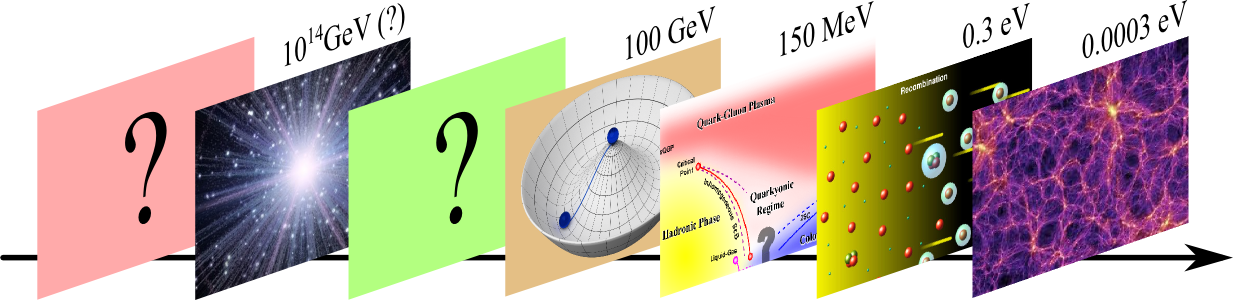
\includegraphics[width=0.8\textwidth]{history}\end{center}

    \titem{
        \item When the universe was 20 picoseconds old (with temperature 100 GeV), a spontaneous symmetry breaking generated mass for known massive fundamental particles.
        \item When the universe was 20 microseconds old (with temperature 150 MeV), free quarks are binded into protons and neutrons. Their binding enery is the main source of mass of atomic matter.
        \item When the universe was 3 minutes old (with temperature 0.1 MeV), light elements, especially helium, are created from protons and neutrons. 
        \item When the universe was 50,000 years old (with temperature 1eV), 
        the universe becomes dominated by non-relativistic matter instead of relativistic radiation.
        \item When the universe was 400,000 years old (with temperature 0.3 eV), the universe become transparent and light for the first time can travel in the universe freely.
        \item In the following billions of years, structures grow in the universe.
        \item Now our universe is about 14 billion years old.
        The universe starts to be dominated by dark energy with $p=-\rho$. We yet need to theoretically and observationally understand the nature of dark energy. 
    }
}

\section{Epilogue: Summary and What's Next}

\textbox{Further reading about the content}{
    \titem{
        \item See Baumann's \href{http://www.damtp.cam.ac.uk/user/db275/Cosmology/Lectures.pdf}{Cosmology} for a detailed introduction of this content.
    }
}

\textbox{What happens next?}{
    Let's first literally discuss what happens next -- what's the future (even fate) of the universe? Now our universe is dominated by dark energy. The energy density of dark energy does not change during the expansion of the universe. As a result, dark energy will become more and more important for the fate of the universe. If the energy density of dark energy is indeed a constant, most galaxies in our present universe will leave our horizon, leaving only $\mathcal{O}(100)$ galaxies around us observable (known as the local group). But we need to further understand dark energy both theoretically and observationally to be more confident about this fate.

    You will find more details about our universe in a course of cosmology. Also, in general relativity there is usually an introduction to cosmology as an application. In-depth study of cosmology usually have close relations to astronomy and high energy physics. 
}

\section{Exercises}

\textbox{E\wref{sec:dynamics-universe}-1 Scale factor as a function of time}{
    For $p=0$ (dust), $p=\rho/3$ (radiation), $p=-\rho$ (dark energy), solve the Friedmann equation to get $a(t)$. Based on your solution, estimate the age of the universe given the value of $H$.
}

\textbox{E\wref{sec:dynamics-universe}-2 我们宇宙的年龄}{
    通过主文饼形图里给的能量分布,估算我们宇宙的年龄。你可以先有一个分析出来的估算然后再运用等式来数学上验证你的估算。
}

\printindex

\end{document}
